\documentclass[]{aiaa-tc}% insert '[draft]' option to show overfull boxes

 \usepackage{varioref}%  smart page, figure, table, and equation referencing
 \usepackage{wrapfig}%   wrap figures/tables in text (i.e., Di Vinci style)
 \usepackage{threeparttable}% tables with footnotes
 \usepackage{dcolumn}%   decimal-aligned tabular math columns
  \newcolumntype{d}{D{.}{.}{-1}}
 \usepackage{nomencl}%   nomenclature generation via makeindex
  \makeglossary
 \usepackage{subfigure}% subcaptions for subfigures
 \usepackage{subfigmat}% matrices of similar subfigures, aka small mulitples
 \usepackage{fancyvrb}%  extended verbatim environments
  \fvset{fontsize=\footnotesize,xleftmargin=2em}
 \usepackage{lettrine}%  dropped capital letter at beginning of paragraph
% \usepackage[dvips]{dropping}% alternative dropped capital package
% \usepackage[colorlinks]{hyperref}%  hyperlinks [must be loaded after dropping]
%\usepackage{makeidx}
\graphicspath{{Images/}}

%AJL SEIT Comment out these two lines for the final submission
\usepackage{draftwatermark}
\SetWatermarkFontSize{5cm} \SetWatermarkScale{6} \SetWatermarkText{\textbf{DRAFT-REMOVE}}


 \title{Preparation of Final Project Summary Report 2015}

 \author{
  Jane B. Smith\thanks{OFFCDT, School of Engineering and Information Technology, ZEIT4500/4501/4297 - delete as appropriate}\
  \\
  {\normalsize\itshape
   UNSW Canberra at ADFA.}\\
  }

 % Data used by 'handcarry' option
 \AIAApapernumber{YEAR-NUMBER}
 \AIAAconference{Conference Name, Date, and Location}
 \AIAAcopyright{\AIAAcopyrightD{YEAR}}

 % Define commands to assure consistent treatment throughout document
 \newcommand{\eqnref}[1]{(\ref{#1})}
 \newcommand{\class}[1]{\texttt{#1}}
 \newcommand{\package}[1]{\texttt{#1}}
 \newcommand{\file}[1]{\texttt{#1}}
 \newcommand{\BibTeX}{\textsc{Bib}\TeX}

%\makeindex

\begin{document}

\maketitle


\begin{abstract}
These instructions give you guidelines for preparing your Final Project Summary Report. Use this document as a template if you are using  \LaTeX\ . Otherwise, use this document as an instruction set. The title of this report should be your project title and should NOT contain the word thesis. This section is the abstract, which should concisely summarise your report including the aim, motivations, methodology and observations (or achievements) and conclusions in a single paragraph. Define all symbols used in the abstract. Do not cite references in the abstract. The abstract should be no more than 400 words in length. The footnote on the first page should list your project course. See  \underbar{http://seit.unsw.adfa.edu.au/ojs/index.php/juer} for past examples of final thesis reports, bearing in mind the length requirements may vary.
\end{abstract}


\tableofcontents
%Anyone know an automated way to do this? Simple as that??!!!!!
%\listoffigures
%\listoftables


\section*{Nomenclature (examples � include units where appropriate)}

%AJL - COMMENT OUT WHEN YOU WANT TO USE THE AUTOMATIC FILLING OF THE AREA - SEE LATER
%\printglossary% creates nomenclature section produced by MakeIndex
\begin{tabbing}
  XXX \= \kill% this line sets tab stop
  $J$ \> Jacobian Matrix \\
  $f$ \> Residual value vector \\
  $x$ \> Variable value vector \\
  $F$ \> Force, [N] \\
  $m$ \> Mass, [kg] \\
  $\Delta x$ \> Variable displacement vector \\
  $\alpha$ \> Acceleration, [m/s\textsuperscript{2}] \\[5pt]
  \textit{Subscript}\\
  $i$ \> Variable number \\
 \end{tabbing}


\section{Introduction (or some other more appropriate heading)}
%\index{}


\lettrine[nindent=0pt]{\textbf{G}}{\textbf{eneral background.}} Autonomous vehicles in general - self driving autopilot etc for personal travel. Relies on mass sensors and data. Wider applications include cognitive assistance and autonomous logistics (refs? Has this been done?). 

\textbf{Other lit review related stuff}

\textbf{Scope and Similar work}. Requirement for robust navigation data. Ability to extend tech requires more agile approach. SIMILAR WORK - MIT local navigation goal \cite{mitLocalNavDriving}. Using CV to align position with map service will allow greater cognitive assistance and automation of tasks without the requirement for significant prior mapping. Benefit -> Augmented reality google maps (eventually autopilot). Automated logistics movements (eg military).

\textbf{Road detection lit review} 
Deep CNN for road detection \cite{deepRoadSegmentation}

\textbf{Autonomous navigation lit review}

\subsection{Project aim}

Trying to rectify GPS location and route polyline with CV data
How is GPS and Nav data stored (polyline)
Workflow : Sim data to Python to analyse, output local nav goal/GPS route in scene
Send back to sim

\subsection{Scope and Deliverables}
Limited to - easily detectable road surface, single lane (Lane detection divorced from project intent but part of it)
Identify intersections and relate to google maps/OSM data

Simulation deliverable

\section{Project management}

\subsection{Project flow}
CV research, Sim development, Lane detection, Intersection detection, Curve matching (splines etc)

\subsection{Gantt Chart discussion}

\section{Current work}

\subsection{Computer Vision? Lane Detection}
Before any effective computer vision approaches can be implemented a robust base of understanding of digital image processing is required (What IS CV, DIP). Background study (textbooks, online course etc)

Intent of CV, what are the outcomes (lane detection, intersection detection)

\subsubsection{Python vs C++}

\subsubsection{Open CV}
Digital Image Processing course, Open CV vs from scratch

\subsubsection{Alternate approaches to lane detection}
CNN discussion with references?

\subsection{Simulation system}
Intent of simulation
IPC

\subsubsection{Simulation engine}
Home rolled vs Unreal (C++ so can talk direct to OpenCV C++) vs Unity 

\subsubsection{IPC}


\section{Results}

\subsection{Computer vision}


\section{Future work}

\subsection{Lane line detection}

Detect the curve of the lane and identify intersections
Curve detection options - sliding window REF LINK %https://www.spiedigitallibrary.org/conference-proceedings-of-spie/0852/0000/Progress-In-Road-Intersection-Detection-For-Autonomous-Vehicle-Navigation/10.1117/12.968232.short?SSO=1


%
%\begin{table}[t] % no placement specified: defaults to here, top, bottom, page
% \begin{center}
%  \caption{Expectations for the Assessment of the Final Project Summary Report \
% (Final Project Summary Report is worth 35\% of the course) }
%  \label{t:scheme_marking}
%  \begin{tabular}{|c|} \hline
%\\
%\textbf{Understanding of the topic: (What and why?)} \\\hline
%�	Has the problem been adequately defined? \\
%�	Has a critical review of the relevant literature been performed? \\
%Note the most important references should be included in this report, whereas \\
%extensive literature reviews where appropriate should be confined to the \\
%Appendices or your separate Project Specific Deliverable. \\
%�	Has the relationship between the project and the literature been adequately defined? \\
%�	Has a clear, appropriate and attainable set of aims been identified? \\
%\\
%\textbf{Methodology (How?)}  \\\hline	
%�	Has a logical process been developed to meet the aims? \\
%�	Has this process been justified? \\
%�	Is the methodology appropriate for the scope of the project? \\
%\\
%\textbf{Analysis}	 \\\hline
%�	Has there been an adequate collection of data/information (or efficient design)? \\
%�	Has appropriate and sufficient analysis been performed to reduce it to a useful form? \\
%�	Have the aims been adequately addressed (if not then have valid reasons been given)? \\
%\\
%\textbf{Discussion, conclusions and recommendations:} \\\hline	
%�	Are they meaningful/worthwhile/significant within the scope of the project? \\
%�	Are they appropriate and adequately justified? \\
%\\
%\textbf{Presentation of the project report:}	 \\\hline
%�	Is the document set out clearly and logically? \\
%�	Does the text clearly explain all aspects of the project to even a non-expert? \\
%�	Has appropriate use been made of figures/tables/charts? \\
%�	Has appropriate and accurate use of referencing been made? \\
%\\
%\textbf{Management}	 \\\hline
%�	There is no requirement for an explicit management document, but it may be \\
%appropriate for you to briefly discuss your learnings in terms of expectations \\
%in the context of your project. \\
%\\
% \\\hline
% \end{tabular}
% \end{center}
%\end{table}



%\begin{figure}[htb]% order of placement preference: here, top, bottom
% 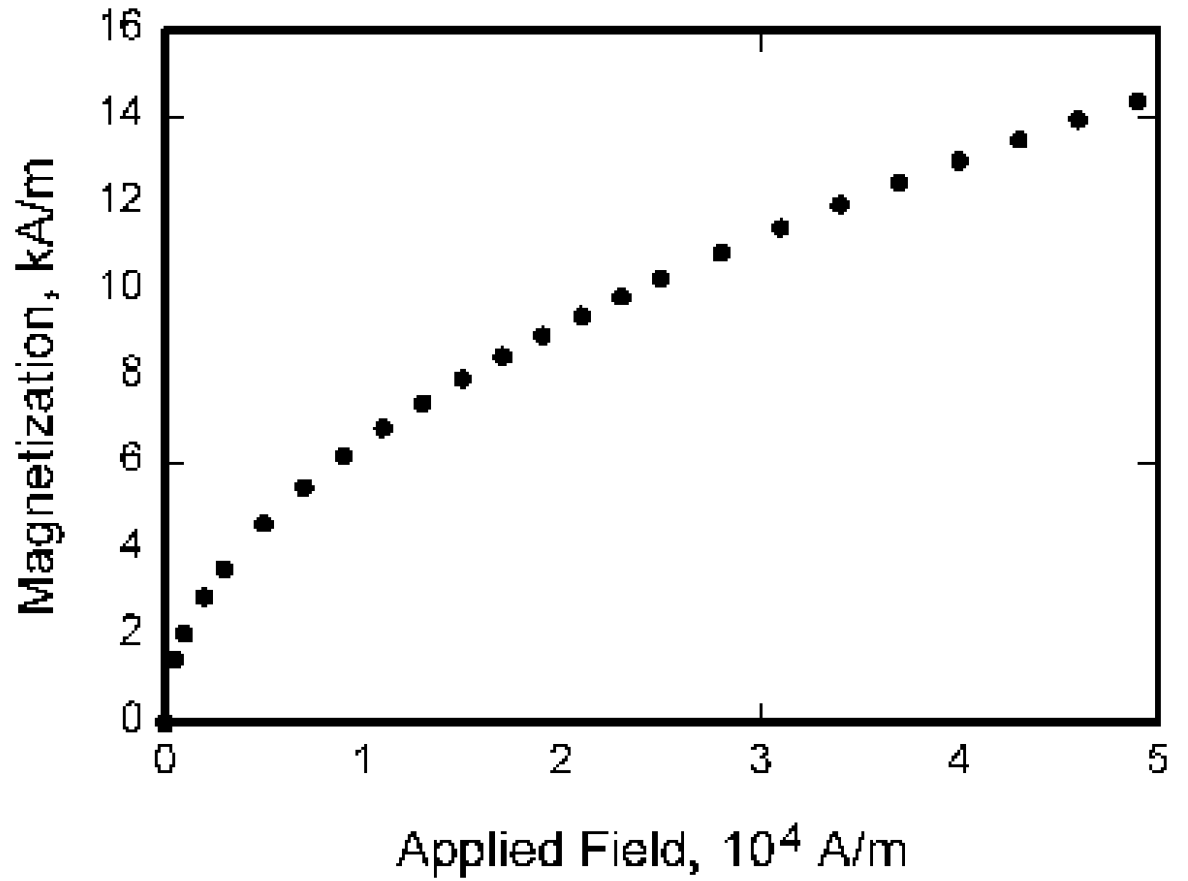
\includegraphics{image_eg.png}
% \caption{Magnetization as a function of applied field, which has
%   borders so thick that they overwhelm the data and for some reason the
%   ordinate label is rotated 90 degrees to make it difficult to
%   read. This figure also demonstrates the dangers of using a bitmap
%   as opposed to a vector image.}
% \label{f:magnetic_field}
%\end{figure}

%
%Sometimes writing meaningless text can be quiet easy, but other times one is hard pressed to keep the words flowing.\footnote{And sometimes things get carried away in endless detail.}
%
%\begin{table}% no placement specified: defaults to here, top, bottom, page
% \begin{center}
%  \caption{Variable and Fixed Coefficient Runge-Kutta Schemes as a
%           Function of Reynolds Number}
%  \label{t:scheme_comparison}
%  \begin{tabular}{rrr}
%       Re & Vary & Fixed \\\hline
%        1 &  868 & 4,271 \\
%       10 &  422 & 2,736 \\
%       25 &  252 & 1,374 \\
%       50 &  151 &   736 \\
%      100 &  110 &   387 \\
%      500 &   85 &   136 \\
%    1,000 &   77 &   117 \\
%    5,000 &   81 &    98 \\
%   10,000 &   82 &    99
%  \end{tabular}
% \end{center}
%\end{table}

%
%\subsubsection{Equations, Numbers, Symbols, and Abbreviations}
%Equations are centered and numbered consecutively, with equation numbers in parentheses flush right, as in  Eq.~(\ref{e:function}) that demonstrates some math
%typesetting.
%
%\begin{equation}
% \label{e:function}
% \int_{0}^{r_{2}} F(r,\varphi) \, dr \, d\varphi =
%    \left[ \sigma r_{2}/(2\mu_{0}) \right] \cdot
%    \int_{0}^{\infty} \exp(-\rho|z_{j}-z_{i}|) \, \lambda^{-1} 
%\end{equation}
%Eq.~(\ref{e:function}) is grand.
%
%
\section{Conclusions}
The conclusions should summarise the main findings of your thesis project including a brief reference to the supporting evidence and to the initial aims. Note that the Conclusions and Recommendations sections are the last sections of the paper that should be numbered. The acknowledgements and references should be listed without numbers.
This had been a brief example of some of the more advanced options available for \LaTeX\ .

\section{Recommendations}
This section should discuss and recommend directions for future work that will build on and extend your research and perhaps resolve some of the issues that you have encountered in your work.

\section*{Acknowledgements}
The Acknowledgements section should be used to briefly thank those individuals or organisations that have assisted you directly in your thesis work whether they be family, friends and colleagues, or technical and academic staff. Note that any external funding source that supported your project should be acknowledged here. 

\section*{Appendices (Separate Document)}
Appendices may used to archive detailed summaries of data such as images, tables and charts and detailed example calculations such as for the estimation of measurement uncertainty. They may also include design drawings. Raw data, or detailed computer programs and files and extensive design drawings, should not be included. Their archiving should be discussed with your supervisor. Any appendices should be submitted as a SINGLE separate document file if referred to in the main text and be listed in the table of contents at the beginning (Note the use of a separate page numbering scheme).

% If you use MakeIndex
%\printindex


% AJL - UNCOMMENT THIS IS PREFERENCE TO THE ABOVE SECTION
%% produces the bibliography section when processed by BibTeX
\bibliography{InterimReferences}
\bibliographystyle{aiaa}



\end{document}

